\chapter{Implementación de \gls{cordic}}
En este capítulo se va a especificar y razonar las herramientas usadas para la implementación de CORDIC y se mostrará tres diferentes implementaciones, además de sus simulaciones y comparativas entre ellas.

\section{Herramientas}
\subsection{Linux}
Todo el trabajo de implementación ha sido realizado dentro de una máquina Linux. Generalmente las herramientas para diseño de nivel hardware comerciales, como Xilinx, son propietarias y desarrolladas exclusivamente para Windows.

Ya que se tiene un buen conocimiento de Linux, se ha optado por buscar herramientas alternativas de código abierto que puedan ofrecer un desarrollo similar a las propietarias.
\subsection{Verilog}
El lenguaje de descripción de hardware (\gls{hdl}) escogido ha sido Verilog/SystemVerilog. Verilog es un subconjunto del lenguaje mas nuevo SystemVerilog. Aunque no se hayan utilizado ninguna nueva parte del diseño, se eligió desde un principio para tener posibilidad de ampliación o necesidad de alguna nueva parte en un futuro.

Ya que en la carrera se realizó prácticas con \gls{vhdl}, se decidió por usar un lenguaje diferente para obtener un amplio conocimiento de los lenguajes principales. Además, Verilog tiene una similitud con el lenguaje C, por lo que puede ser mas atractivo si se tiene algún conocimiento de este lenguaje.

\subsection{Verilator}
La herramienta elegida para la compilación y comprobación del funcionamiento de \gls{cordic} ha sido Verilator. Esta herramienta es gratuita y de código abierto. Además esta desarrollada para Ubuntu, pero funciona en casi todas las distribuciones de Linux. En concreto, todo el desarrollo ha sido realizado en dos máquinas con Arch Linux.

Su principales características son la compilación del código de Verilog a C++ o SystemC. Este código es mucho mas optimizado y permite un mejor rendimiento a la hora de simular. Además, permite diseñar \textit{testbench} en C++, por lo que puede facilitar mucho la forma de desarrollar si se tiene un conocimiento de C++.

Aunque no se vaya a usar en gran parte las ventajas que ofrece Verilator, podemos sacar de provecho para dar una entrada a futuros proyectos.

\section{Configuración de Verilator}
Para compilar nuestro código Verilog/SystemVerilog necesitaremos usar el comando \textit{verilator}. Un ejemplo básico sería el siguiente:

\begin{lstlisting}
verilator -Wall --cc cordic.sv
\end{lstlisting}

Después de ejecutar el comando, Verilator crea una carpeta llamada \textit{obj\_dir}, donde podemos encontrar un fichero Makefile, que en este caso su nombre sería \textit{Vcordic.mk}. Este makefile crea el ejecutable final.

Para poder implementar los testbench en C++, se debe de inicializar Verilator con las variables de \textit{argc} y \textit{argv}. Para poder acceder a las entradas y salidas de Verilog necesitamos crear una instancia de nuestro módulo a probar. En este caso sería un tipo \textit{Vcordic}, el cual esta incluido en "obj\_dir/Vcordic.h"

\begin{lstlisting}[caption={Definición de una TestBench de Verilator}] 
class TestBench{
     unsigned long m_tickcount;
     Vcordic *m_core;
     VerilatedVcdC   *m_trace;
     
     TestBench(void){
         m_core = new Vcordic;
         m_tickcount = 0l;
         Verilated::traceEverOn(true);
     }
     
	...
};
\end{lstlisting}

Dentro de la definición del \textit{TestBench} tenemos un tipo \textit{Vcordic*}, el cual permitirá acceder a las variables del módulo. La variable de tipo \textit{unsigned long}, \textit{m\_tickcount}, permite tener un tiempo de referencia interno en nuestra $testbench$.

La última línea del constructor es una llamada a Verilator para poder llamar a cualquier función para trazar las señales del módulo para luego ser usadas en un programa como \textit{GTKWave}.

Para poder trazar las señales necesitamos definir dos funciones: \textit{opentrace()} y \textit{close()}.

\begin{lstlisting}[caption={Definición de funciones para trazar la simulación.}]
 virtual void opentrace(const char *name) {
     m_trace = new VerilatedVcdC;
     m_core->trace(m_trace, 99);
     m_trace->open(name);

 }

 virtual void close(void) {
     m_trace->close();
     delete m_trace;
     m_trace = NULL;
 }
\end{lstlisting}

Estas dos funciones se usarán dentro de la función \textit{main()} antes y después de pasar por el bucle principal.

Ahora necesitamos crear las funciones de $tick()$ y $reset()$.

\begin{lstlisting}[caption={Definición de funciones \textit{reset()} y \textit{tick()}}]
  virtual void reset(void){

     m_core->iReset = 1;
     this->tick();
     m_core->iReset = 0;
  }

 virtual void tick(void){
     m_tickcount++;

     m_core->iClock = 0;
     m_core->eval();
     
     if(m_trace) 
         m_trace->dump(10*m_tickcount-2);

     m_core->iClock = 1;
     m_core->eval();
     
     if(m_trace)
         m_trace->dump(10*m_tickcount);
     

     m_core->iClock = 0;
     m_core->eval();
     
     if (m_trace) {
         m_trace->dump(10*m_tickcount+5);
         m_trace->flush();
     }
     
 }
\end{lstlisting}

La función $tick()$ incrementa el tiempo de referencia interno, evalúa cualquier lógica combinatoria con una función interna de Verilator, $eval()$, ya que es posible de que el valor haya cambiado antes de haber sido llamado $tick()$. Posteriormente cambia el reloj $iClock$ a 1 y evalúa el estado y vuelve a cambiar el reloj a 0.

Además, la función \textit{tick()} tiene unas llamadas al trazado de las señales si el usuario lo ha inicializado con las llamadas apropiadas anteriormente.

La función reset() cambia la entrada de $iReset$ a 1, evalúa el módulo con un $tick()$ y vuelve a cambiar la entrada a 0.

A partir de ahora, solo necesitamos tener un bucle en nuestra función main para probar el módulo.

\section{Implementación básica}
Ya que \gls{cordic} tiene la ventaja de ser muy fácil de implementar en hardware, una implementación básica de \gls{cordic}  nos permite realizar

Las entradas de nuestro módulo $iX, iY, iAngle, iClock$ y $iReset$. Las salidas son $oX$ y $oY$. Inicialmente todos las entradas y salidas son enteros de 32 bits.

\begin{lstlisting}[caption={Módulo \gls{cordic}}]
module cordic(iClock, iReset, iAngle, iX, iY, oX, oY);
\end{lstlisting}

Antes de iniciar \gls{cordic}, necesitamos conocer en que cuadrante se encuentra el ángulo de entrada. Cada artículo citado ha tomado una decisión propia a la hora de abarcar este problema. Una manera fácil de saber el cuadrante en el que se encuentra es hacer el módulo de $2\pi$ radianes y empaquetando el valor del ángulo en un registro de 32 bits. En este caso, 0 grados se traduce a un valor de todos los bits a 0 y un valor de 359.999... sería todo los bits a 1, aunque en nuestro caso solo hay valores enteros. Esta transformación tiene que ser realizada por el usuario antes de pasarla por la entrada $iAngle$. Aunque esto es posible implementarlo dentro del módulo o uno externo, por simplificar se ha decidido cambiar el ángulo en el \textit{testbench} para centrarse en \gls{cordic}.

Ahora solo tenemos que leer los 2 bits mas significativos para saber en que cuadrante se encuentra el ángulo. Este paso solo se ejecuta al principio del algoritmo.
\begin{lstlisting}[caption={Pre-rotación de iAngle pasado por el usuario.}]
 begin
     case(quadrant)
         2'b00,
         2'b11: 
         begin
             X <= iX;
             Y <= iY;
             Z <= iAngle;
         end

         2'b01:
         begin
             X <= -iY;
             Y <= iX;
             Z <= {2'b00,iAngle[29:0]};
         end

         2'b10:
         begin
             X <= iY;
             Y <= -iX;
             Z <= {2'b11,iAngle[29:0]};
         end
     endcase
 end

\end{lstlisting}
La LUT de ángulos predefinidos de $\arctan(2^{-i})$ tiene el mismo formato que $iAngle$.
\begin{lstlisting}[caption={Tabla de $\arctan$.}]
wire signed [31:0] atan_angle [0:30]

 assign atan_angle[00] = 32'h20000000; // arctan(2^0)
 assign atan_angle[01] = 32'h12E4051D; 
 assign atan_angle[02] = 32'h9FB385B; 
 ...
 assign atan_angle[28] = 32'h2;
 assign atan_angle[29] = 32'h1;
 assign atan_angle[30] = 32'h0;
\end{lstlisting}

Se ha definido un total de 31 valores, aunque como se verá mas tarde no van a ser necesarios todos los valores de la tabla para conseguir un valor cercano al real.

Ahora definimos 3 tipos registros y 3 tipo $wire$.

\begin{lstlisting}[caption={Registros y $wire$ para operar con \gls{cordic}}]
 reg signed [IOWidth-1:0] X;
 reg signed [IOWidth-1:0] Y;
 reg signed    [31:0] Z; 
 
 wire signed [31:0] X_shr = X >>> i-1;
 wire signed [31:0] Y_shr = Y >>> i-1;
 wire Z_sign = Z[31];  
\end{lstlisting}

Estos registros nos servirán para guardar los resultados de cada micro-rotación de \gls{cordic} y los $wire$ guardan la operación de movimiento de bits de $X$ e $Y$ y el signo de $Z$.

\begin{lstlisting}[caption={Bucle principal de \gls{cordic}}]
 begin
     X <= Z_sign ? X + Y_shr         : X - Y_shr;
     Y <= Z_sign ? Y - X_shr         : Y + X_shr;
     Z <= Z_sign ? Z + atan_angle[i-1] : Z - atan_angle[i-1];
 end
\end{lstlisting}

Este sería el código representando las fórmulas finales que se han obtenido a la hora de despejar la función $\textbf{R}$.

\subsection{Testbench de \gls{cordic}}
Para probar el funcionamiento, utilizaremos la \textit{testbench} definida anteriormente. Dentro de nuestro fichero "main.cpp" necesitamos inicializar Verilator con la siguiente línea:

\begin{lstlisting}
Verilated::commandArgs(argc,argv);
\end{lstlisting}

Despues de incluir el fichero "TestBench.h" en el "main.cpp", debemos de crear un tipo \textit{TestBench} y cargar las variables de la clase con los valores deseados.

\begin{lstlisting}[caption={Creación del tipo TestBench y entrada de valores desde C++ al módulo de \gls{cordic} en Verilog}]
 TestBench *tb = new TestBench();

 const float K = 1.646760;
 int32_t angle = atoi(argv[3]);
 int32_t X = atoi(argv[1]);
 int32_t Y = atoi(argv[2]);

 tb->m_core->iX = X / K;
 tb->m_core->iY = Y / K;
 tb->m_core->iAngle = (pow(2,32)*angle)/360;
\end{lstlisting} 

Después de crear el objeto \textit{TestBench}, introducimos los valores de X e Y, dividiéndolo antes por el factor $K$. El ángulo es transformado a un valor módulo de 360 y elevado a $2^{32}$ para que tenga el mismo formato que la tabla de $\arctan$ que tenemos predefinida en nuestro código Verilog.

El factor $K$ es extraído de los valores a pasar antes de la ejecución. Dependiendo de las especificaciones esto se podría dejar con el factor $K$ si no fuera necesario.

Finalmente, iniciamos la traza y el bucle para ir ciclo por ciclo en nuestra ejecución.

\begin{lstlisting}[caption={Bucle principal de main.cpp}]
 tb->opentrace("test.vcd");
 for(int x=0;x<NUM_TICKS;x++)
 {
     tb->tick();
     ...
 }
 tb->close();
\end{lstlisting}

Este \textit{testbench} es prácticamente idéntico en todas las implementaciones que se van a realizar, por lo que solo se va a comentar en la sección de \gls{cordic} básico.

Ahora se mostrará un ejemplo de una \textit{testbench} con los siguientes parámetros.
\begin{lstlisting}
./cordic 1000 0 130
\end{lstlisting}

El primer valor se refiere a $X$, el segundo al valor $Y$ y el último al ángulo que queremos rotar. El valor final será multiplicado por 1000 para obtener un resultado deseado, donde se pueda ver que realmente se realizan las operaciones de seno y coseno. El valor $Y$, según la especificación del método, tiene que tener un valor 0 para obtener el seno y coseno (véa la tabla \ref{table:2009-CORDIC-Configurations}).

\begin{lstlisting}
tick = 0
cos = 0
sin = 607

tick = 1
cos = -607
sin = 607

tick = 2
cos = -304
sin = 911

tick = 3
cos = -531
sin = 835
Este es un

tick = 4
cos = -635
sin = 768

tick = 5
cos = -683
sin = 728

tick = 6
cos = -661
sin = 750

tick = 7
cos = -650
sin = 761

tick = 8
cos = -645
sin = 767

tick = 9
cos = -643
sin = 770

tick = 10
cos = -644
sin = 768

tick = 11
cos = -644
sin = 767

tick = 12
cos = -644
sin = 766

tick = 13
cos = -644
sin = 767

tick = 14
cos = -644
sin = 766

tick = 15
cos = -644
sin = 767

tick = 16
cos = -644
sin = 768
...
\end{lstlisting}

La salida de seno y coseno muestran los registros $X$ e $Y$. A diferencia de las siguientes implementaciones, esta te devuelve un valor distinto de 0 desde el primer ciclo, ya que se esta operando siempre sobre ese valor.

Sobre el \textit{tick} 16, el valor se aproxima mucho al valor real de seno y coseno, por lo que no tiene mucho sentido realizar mas micro-rotaciones, ya que los valores menos significativos se encuentran ahí.

Para ver las salidas por GTKWave, vea la figura \ref{graf:salida_gtkwave_basico}.

\section{Implementación \textit{pipeline}}
El $pipelining$ es un método clásico de conectar elementos de procesamiento en series para  mejorar el rendimiento de los sistemas. Muchos artículos de \gls{cordic} proponen un sistema con algún tipo de $pipelining$. En este punto se mostrará un ejemplo de $pipelining$ básico que se puede implementar con el código implementado en el punto anterior.

La operación de micro-rotación que realiza \gls{cordic} puede ser diseñada de forma que los valores se muevan en serie por todas las etapas del método. Para esto necesitamos el mismo número de registros que etapas para guardar los valores intermedios.

\begin{lstlisting}[caption={Registros de \gls{cordic} ampliados para \textit{pipelining}}]
localparam ETAPAS = 16;

 reg signed [IOWidth:0] X [0:ETAPAS-1];
 reg signed [IOWidth:0] Y [0:ETAPAS-1];
 reg signed    [31:0] Z [0:ETAPAS-1];

\end{lstlisting}

Verilog tiene un constructor llamado $generate$. Sus funciones principales son la instanciación de los $items$ del módulo, cambio de la estructura del diseño a partir de los parámetros pasados por Verilog y verificación funcional de los módulos. En nuestro caso lo usaremos para generar todas las etapas de ejecución del método \gls{cordic}.

Los bloques de $generate$ son generados antes de la ejecución del circuito, ya que no es posible añadir o eliminar hardware en tiempo de ejecución.

Para generar los bloques necesitamos una variable $genvar$. Además, todos los $wire$ que asignan el tipo de signo del ángulo y los movimientos de bits son también generados dentro de $generate$.

\begin{lstlisting}[caption={Ejecución principal de \gls{cordic} con \textit{pipelining}}]
 genvar i;
 generate
 for (i = 0;i < (ETAPAS-1);i=i+1) 
 begin
     wire        Z_sign;
     wire signed [IOWidth:0] X_shr, Y_shr;

     assign X_shr = X[i] >>> i; 
     assign Y_shr = Y[i] >>> i;

     assign Z_sign = Z[i][31];
         
     always @(posedge iClock)
     begin
         // add/subtract shifted data
         X[i+1] <= Z_sign ? X[i] + Y_shr         : X[i] - Y_shr;
         Y[i+1] <= Z_sign ? Y[i] - X_shr         : Y[i] + X_shr;
         Z[i+1] <= Z_sign ? Z[i] + atan_angle[i] : Z[i] - atan_angle[i];
     end 
 end     
 endgenerate
\end{lstlisting}

Como se puede observar, el espacio que ocupa un \gls{cordic} con $pipelining$ es mayor que el básico, ya que necesitamos generar el mismo número de registros que de etapas en nuestro \textit{pipeline}, pero tenemos la ventaja de una mejora del $throughput$. A partir del ciclo 16 estamos recibiendo cada ciclo un nuevo resultado.

Ya que esta implementaciones no han sido probadas en hardware real y solamente simuladas, hay algunos aspectos que no se tienen en cuenta que si pueden ocurrir en un sistema real, como por ejemplo en una \gls{fpga}.

\begin{itemize}
	\item No hay una forma de comprobar que los resultados obtenidos son válidos. Esto viene del hecho de que el módulo va a estar ejecutándose continuamente cada ciclo sin tener en cuenta si su entrada es válida o no. Una forma de arreglar esto es mediante una entrada \textit{Clock Enable} (CE), la cual esta conectada a todos las etapas y es la única que permite mover los datos de un etapa a otra.
	
	\item Es posible que el dispositivo al que estamos transmitiendo no esta preparado para recibir los datos. La solución a este problema es tener conectada una entrada de \textit{BUSY}, que dependiendo del tipo de transmisor que sea tendrá una especificación u otra. Para que se pueda transmitir datos de forma correcta, \textit{BUSY} tendría un valor 0 y \textit{Clock Enable} un valor 1.
\end{itemize}

\subsection{Testbench de CORDIC \textit{pipeline}}
A continuación se va a mostrar la salida del \textit{Testbench}. En esta \textit{testbench} se ha optado por pasar cada ciclo un nuevo ángulo, comenzando por el 10, para mostrar el funcionamiento del \textit{pipelining}. Cada ciclo después del \textit{tick} 15 se está devolviendo un nuevo valor. Para ver las salidas por GTKWave, vea la figura \ref{graf:salida_gtkwave_pipeline}.

\begin{lstlisting}
tick = 0

cos = 0
sin = 0
tick = 1

cos = 0
sin = 0
tick = 2

cos = 0
sin = 0
tick = 3

cos = 0
sin = 0
tick = 4

cos = 0
sin = 0
tick = 5

cos = 0
sin = 0
tick = 6

cos = 0
sin = 0
tick = 7

cos = 0
sin = 0
tick = 8

cos = 0
sin = 0
tick = 9

cos = 0
sin = 0
tick = 10

cos = 0
sin = 0
tick = 11

cos = 0
sin = 0
tick = 12

cos = 0
sin = 0
tick = 13

cos = 0
sin = 0
tick = 14

cos = 0
sin = 0
tick = 15

cos = 984
sin = 175
tick = 16

cos = 935
sin = 346
tick = 17

cos = 864
sin = 499
tick = 18

cos = 766
sin = 644
tick = 19

cos = 644
sin = 766
tick = 20
\end{lstlisting}

Como se comento en la sección anterior, la implementación \textit{pipeline} tiene el mismo número de registros que de etapas por las que pasa el método, por lo que en las primeras ejecuciones no vamos a recibir ningun valor, ya que el método aún no ha llegado a esa etapa.

Se puede observar una clara mejora al \gls{cordic} básico, ya que no necesitamos esperar al resultado de una entrada antes de enviar otra, si no que cada ciclo podemos dar un nuevo valor a tratar.


\section{Implementación con punto flotante}
Para la implementación de punto flotante necesitamos realizar algunas modificaciones al tipo de datos que estamos tratando. Las entradas \textit{iX} y \textit{iY} eran enteros con signo de 32 bits. En esta implementación necesitamos usar un nuevo formato de punto fijo, en concreto el formato Q.

El formato Q(m,n) nos permite operar con el mismo hardware que un entero, por lo que reduce la complejidad de operar directamente con el estándar \gls{ieee} 754. En concreto, el formato es Q(8,24), con 8 bits de entero y 24 bits fraccionarios.

En el código de "main.cpp", tenemos que modificar la línea de entrada de valores \textit{iX} y \textit{iY} para que estén acorde al formato Q(8.24). Para ello necesitamos elevar el valor que pasamos por argumento a $2^{24}$.

\begin{lstlisting}[caption={Cambios de entrada de valores de C++ a Verilog en la implementación de Punto Flotante}]
 ...
 tb->m_core->iX = (X * pow(2,24)) / K;  
 tb->m_core->iY = (Y * pow(2,24)) / K;
 ...
\end{lstlisting}

Dentro del código de Verilog, el bucle principal de micro-rotaciones y el movimiento de bits se queda igual que en las otras implementaciones. La división en formato fijo se puede realizar si el divisor es $2^i$, por lo que podemos hacer el movimiento de bits necesario por \gls{cordic} sin problemas. Hay otra manera de dividir, que sería la multiplicación por un número decimal, con el cual conseguiríamos una división, pero añadir una multiplicación al bucle de \gls{cordic} llevaría a mayor complejidad hardware y peores tiempos.

A la hora de obtener el resultado necesitamos transformar el valor en el estándar del \gls{ieee} 754. Para ello se ha diseñado una máquina de estado finita (\gls{fsm}).

Una forma muy general de diseñar una \gls{fsm} es mediante dos registros: \textit{current\_state} y \textit{next\_state}. Después, un parámetro es declarado por cada estado que se encuentre en el diagrama de estados. Los parámetros necesitan un valor en concreto para poder usar su nombre declarado en las asignaciones siguientes.

\begin{lstlisting}[caption={Registros para controlar los estádos y parámetros locales de estado para controlar la máquina de estado finita.}]
reg [2:0]  current_state = w_normal_op, next_state;

localparam      w_normal_op = 3'b000,
                w_check_sign = 3'b001,
                w_bit_shift_count = 3'b010,
                w_to_fp = 3'b011,
                w_reset = 3'b100;

\end{lstlisting}

Aquí podemos ver una declaración de 2 registros mencionados anteriormente con 3 bits cada uno, para poder codificar un máximo de $2^3$ estados diferentes. Al crear los parámetros tenemos que asignarles un valor de 3 bits.

Primero se va a comentar una idea general de cada estado y luego se entrará en los detalles del funcionamiento. El modo de operación de la \gls{fsm} es la siguiente:

\begin{itemize}
	\item \textit{w\_normal\_op} es el modo de operación normal de \gls{cordic} con \textit{pipelining}. La \gls{fsm} se encuentra en este modo hasta encontrar con un nuevo valor en el último registro de nuestra \textit{pipeline}, la cual se refiere al valor final calculado por gls{cordic}.
	
	\item \textit{w\_check\_sign} es un estado intermedio que transforma los valores negativos de complemento a 2 a un valor binario normal. Antes de convertirlo se guarda el signo, que viene representado por el último bit (31).
	
	\item \textit{w\_bit\_shift\_count} calcula el movimiento de bits que se debe de realizar para alinear los bits con la mantisa.
	
	\item \textit{w\_to\_fp} realiza la transformación final a punto flotante y reinicia todos los valores intermedios que se han usado para operar correctamente.
	
	\item \textit{w\_reset} reinicia el módulo poniendo todos los registros, entradas y salidas a 0.
	
\end{itemize}

Una \gls{fsm} tiene los llamados \textit{state memory}, \textit{next state logic} y \textit{output logic}.

El primer estado de memoria (\textit{state memory}) es el que se dedica simplemente a actualizar el estado cada vez que hay una subida de reloj.

\begin{lstlisting}[caption={\textit{state memory} de \gls{cordic}}]
always@(posedge iClock or negedge iReset)
 begin: STATE_MEMORY
     if(iReset == 1'b1)
         current_state <= w_reset;
     else
         current_state <= next_state;
 end
\end{lstlisting}

El siguiente bloque es el \textit{next state logic}. Aquí se suele utilizar el \textit{case} para controlar a que estado pasar. Generalmente se recomienda hacer uso del \textit{default} por si hay un error inesperado.

Este bloque solo es activado por el registro \textit{current\_state}, lo que convierte esta \gls{fsm} una máquina de Moore, ya que el sistema cambia por un cambio en el estado, independiente de cualquier otra entrada. De no ser así la \gls{fsm} sería una máquina de Mealy y se incluiría dentro de la lista de sensibilidad otras entradas dependientes.

\begin{lstlisting}[caption={Código de la \textit{next state logic} de la \gls{fsm}}]
always@(current_state)
 begin: NEXT_STATE_LOGIC
     case(current_state)
         default:
         begin
         end
         
         w_normal_op:
             begin
                 if(last_x_value != X[ETAPAS-1] || last_y_value != Y[ETAPAS-1] begin
                     next_state = w_check_sign;
                 end
             end

         w_check_sign:
             if(sign_checked) begin
                 next_state = w_bit_shift_count;
             end
         w_bit_shift_count:
             if(tempXOut[bitmov_x] == 1 && tempYOut[bitmov_y] == 1 ) begin
                 next_state = w_to_fp;
             end
         w_to_fp:
             if(fp_out) begin
                 next_state = w_normal_op;
             end
     endcase
 end
\end{lstlisting}

Este bloque realiza las siguientes funciones:

\begin{itemize}
	\item \textit{w\_normal\_op} Observa si el valor $x$ o $y$ anterior coincide con los que hay actualmente en el último registro del método \gls{cordic}. De no ser así significa que el usuario ha dado un nuevo valor de entrada al módulo y, por tanto, necesitamos pasar por la conversión a punto flotante.
	
	\item \textit{w\_check\_sign} En el momento que se recibe un \textit{sign\_checked} pasamos al contador del número de bits a mover.
	
	\item \textit{w\_bit\_shift\_count} Se observa si el bit en una posición determinada es 1 de las dos variables temporales que se manipulan dentro de la \gls{fsm}. Si es así se pasa a la transformación de punto fijo a flotante.
	
	\item \textit{w\_to\_fp} Espera hasta que el registro \textit{fp\_out} sea asignado a 1. En ese momento la transformación a punto flotante se ha finalizado.
\end{itemize} 

Ahora vamos a pasar al bloque de \textit{output logic}. Este bloque realiza todas las operaciones necesarias para convertir a punto flotante.

\begin{lstlisting}[caption={Código de \textit{output logic} de la \gls{fsm}}]
always @(current_state)
begin: OUTPUT_LOGIC 
  case(current_state)
      w_normal_op,

      w_check_sign:
      begin
          fp_out = 0;
          fpX_out = 0;
          fpY_out = 0;

          tempXOut = X[ETAPAS-1];
          sign_x = tempXOut[31];

          tempYOut = Y[ETAPAS-1];
          sign_y = tempYOut[31];


          if(tempXOut[31] == 1)
          begin
              \textit{w\_normal\_op}tempXOut = ~(tempXOut-1);
          end


          if(tempYOut[31] == 1)
          begin
              tempYOut = ~(tempYOut-1);
          end

          sign_checked = 1;
      end

      w_bit_shift_count:
      begin
          sign_checked = 0;
          if(tempXOut[bitmov_x] != 1 )
          begin
              bitcount_x = bitcount_x + 1;
              bitmov_x = bitmov_x - 1;
          end
          if(tempYOut[bitmov_y] != 1)
          begin
              bitcount_y = bitcount_y + 1;
              bitmov_y = bitmov_y - 1;
          end
      end

      w_to_fp:
      begin
          if(!fp_out)
          begin

              if(tempXOut[30:23] != 0) begin
                  tempXOut = tempXOut >> (8-bitcount_x);
              end
              else begin
                  tempXOut = tempXOut << ~((8-bitcount_x)-1);
              end

              tempXOut[30:23] = (127 + (8 - (bitcount_x+1)));
              tempXOut[31] = sign_x;
              fpX_out = tempXOut;
              bitmov_x = 31;
              bitcount_x = 0;

              if(tempYOut[30:23] != 0) begin
                  tempYOut = tempYOut >> (8 - bitcount_y);
              end
              else begin
                  tempYOut = tempYOut << ~((8 - bitcount_y)-1);
              end

              tempYOut[30:23] = (127+(8 - (bitcount_y+1)));
              tempYOut[31] = sign_y;
              fpY_out = tempYOut;
              bitmov_y = 31;
              bitcount_y = 0;
              fp_out = 1;
          end
      end
      default:
          begin
          end

  endcase

     end

\end{lstlisting}

Las funciones realizadas por este bloque son las siguientes:

\begin{itemize}	
	\item \textit{w\_check\_sign} Reinicia los valores de las ejecuciones pasadas. Posteriormente guarda en dos registros los signos de la $X$ e $Y$. Por último se hace una transformación de complemento a 2 a binario normal si el valor fuese negativo y se pone el registro \textit{sign\_checked} a 1.
	
	\item \textit{w\_bit\_shift\_count} Hace recuento del movimiento de bits que se debe de realizar para ajustarlo con la mantisa. Los valores \textit{bitmov} y \textit{bitcount} inicialmente tienen un valor de 31 y 0 respectivamente. El contador de $X$ e $Y$ se detiene en el momento que encuentra un 1 en la posición que este actualmente.
	
	\item \textit{w\_to\_fp} La variable \textit{tempXOut} y \textit{tempYOut} tiene que ser ajustada a la mantisa de un \gls{ieee} 754 de 32 bits, la cual son los 23 bits menos significativos. Ya que el movimiento de bits puede ser a la derecha o izquierda, dependiendo de la magnitud del valor, necesitamos tener en cuenta los dos casos.
	
	Despues de ajustar la mantisa necesitamos guardar en el exponente. Para ello tenemos que tener en cuenta el número de movimiento de bits que se ha realizado anteriormente y sumar el sesgo del exponente, que para un valor de 32 bits es 127. Esta operación se hace para $X$ e $Y$
	
	Finalmente, reiniciamos los valores y volvemos al estado \textit{w\_normal\_op}.
\end{itemize}

La salida de los valores $X$ e $Y$ no van directamente asignados desde los registros finales de la última etapa de CORDIC como en las anteriores implementaciones. Las salidas son asignadas en el último estado de la \gls{fsm} y reiniciadas a 0 en el momento que hay una nueva operación de transformación a punto flotante.

\begin{lstlisting}[caption={Cambio en las asignaciones de las salidas de CORDIC en punto flotante}]
assign oY = fpY_out;
assign oX = fpX_out;
\end{lstlisting}

El \textit{pipelining} además tiene que detenerse en el momento que hay un nuevo valor a procesar, por lo que necesitamos detener el bucle principal de CORDIC hasta que termine la \gls{fsm}.

\begin{lstlisting}[caption={Cambio en el bucle principal de CORDIC.}]
 if(next_state == w_normal_op) begin

     X[i+1] <= Z_sign ? X[i] + Y_shr         : X[i] - Y_shr;
     Y[i+1] <= Z_sign ? Y[i] - X_shr         : Y[i] + X_shr;
     Z[i+1] <= Z_sign ? Z[i] + atan_angle[i] : Z[i] - atan_angle[i];
 end
 
 else begin
     last_x_value <= X[ETAPAS-1];
     last_y_value <= Y[ETAPAS-1];
 end
\end{lstlisting}

Simplemente comprobamos si el siguiente estado es \textit{w\_normal\_op} y de no ser así, detenemos toda la \textit{pipeline} de CORDIC.
\subsection{Testbench de CORDIC punto flotante con \textit{pipelining}}
Este \textit{testbench} es muy parecido a la implementación con \textit{pipelining}. Cada ciclo introducimos una nueva entrada. El primer valor es introducido como argumento de la ejecución del programa, que es:

\begin{lstlisting}
./cordic 1 0 45
\end{lstlisting}

Los demas valores empiezan por un ángulo de 10.

\begin{lstlisting}
// ticks omitidos que devuelven un valor 0.
tick = 1
tick = 2
...
tick = 18
tick = 19
cos = 0.707117
sin = 0.707096
tick = 20
...
tick = 23
cos = 0.984809
sin = 0.17364
tick = 24
...
tick = 27
cos = 0.939708
sin = 0.341977
tick = 28
...
tick = 31
cos = 0.866003
sin = 0.500039
tick = 32
...
tick = 35
cos = 0.766029
sin = 0.642806
tick = 36
...
tick = 39
cos = 0.642806
sin = 0.766029
tick = 40
...
tick = 43
cos = 0.500039
sin = 0.866003
tick = 44
...
tick = 47
cos = 0.341977
sin = 0.939708
tick = 48
...
tick = 51
cos = 0.17364
sin = 0.984809
tick = 52
...
tick = 55
cos = -1.3113e-05
sin = 1
tick = 56
...
tick = 59
cos = -0.17364
sin = 0.984809
tick = 60
...
tick = 63
cos = -0.341977
sin = 0.939709
tick = 64
...
tick = 67
cos = -0.500039
sin = 0.866003
...

\end{lstlisting}

A diferencia de un \textit{pipelining} estándar, necesitamos transformar el valor en punto flotante, por lo que tardamos 4 ciclos mas en devolver un resultado. Aun así, tenemos un \textit{throughput} mas alto que un \gls{cordic} tradicional y una mejor precisión en los valores devueltos.

Como tambien se puede observar, algunos valores se tienen que aproximar a su resultado real. En el \text{tick} 55 los valores representados son seno y coseno de 90. El coseno es lo suficientemente pequeño para ser considerado 0. Para ver las salidas por GTKWave, vea la figura \ref{graf:salida_gtkwave_fp}.

En este \textit{testbench} se ha optado por no multiplicar los valores por 1000, pero se puede hacer de la misma forma que en los otros \textit{testbench} y nos dará un resultado mas preciso.

En la figura \ref{graf:real_error} podemos ver el error producido en cada etapa del cálculo de un valor. A partir de la micro-rotación 26 el error es idéntico en cada etapa. Todos las implementaciones fueron probadas con sólo 16 etapas para facilitar el desarrollo, pero pueden ampliarse perfectamente a más si es necesario una menor tasa de error.
\begin{figure}[ht]
	\centering
	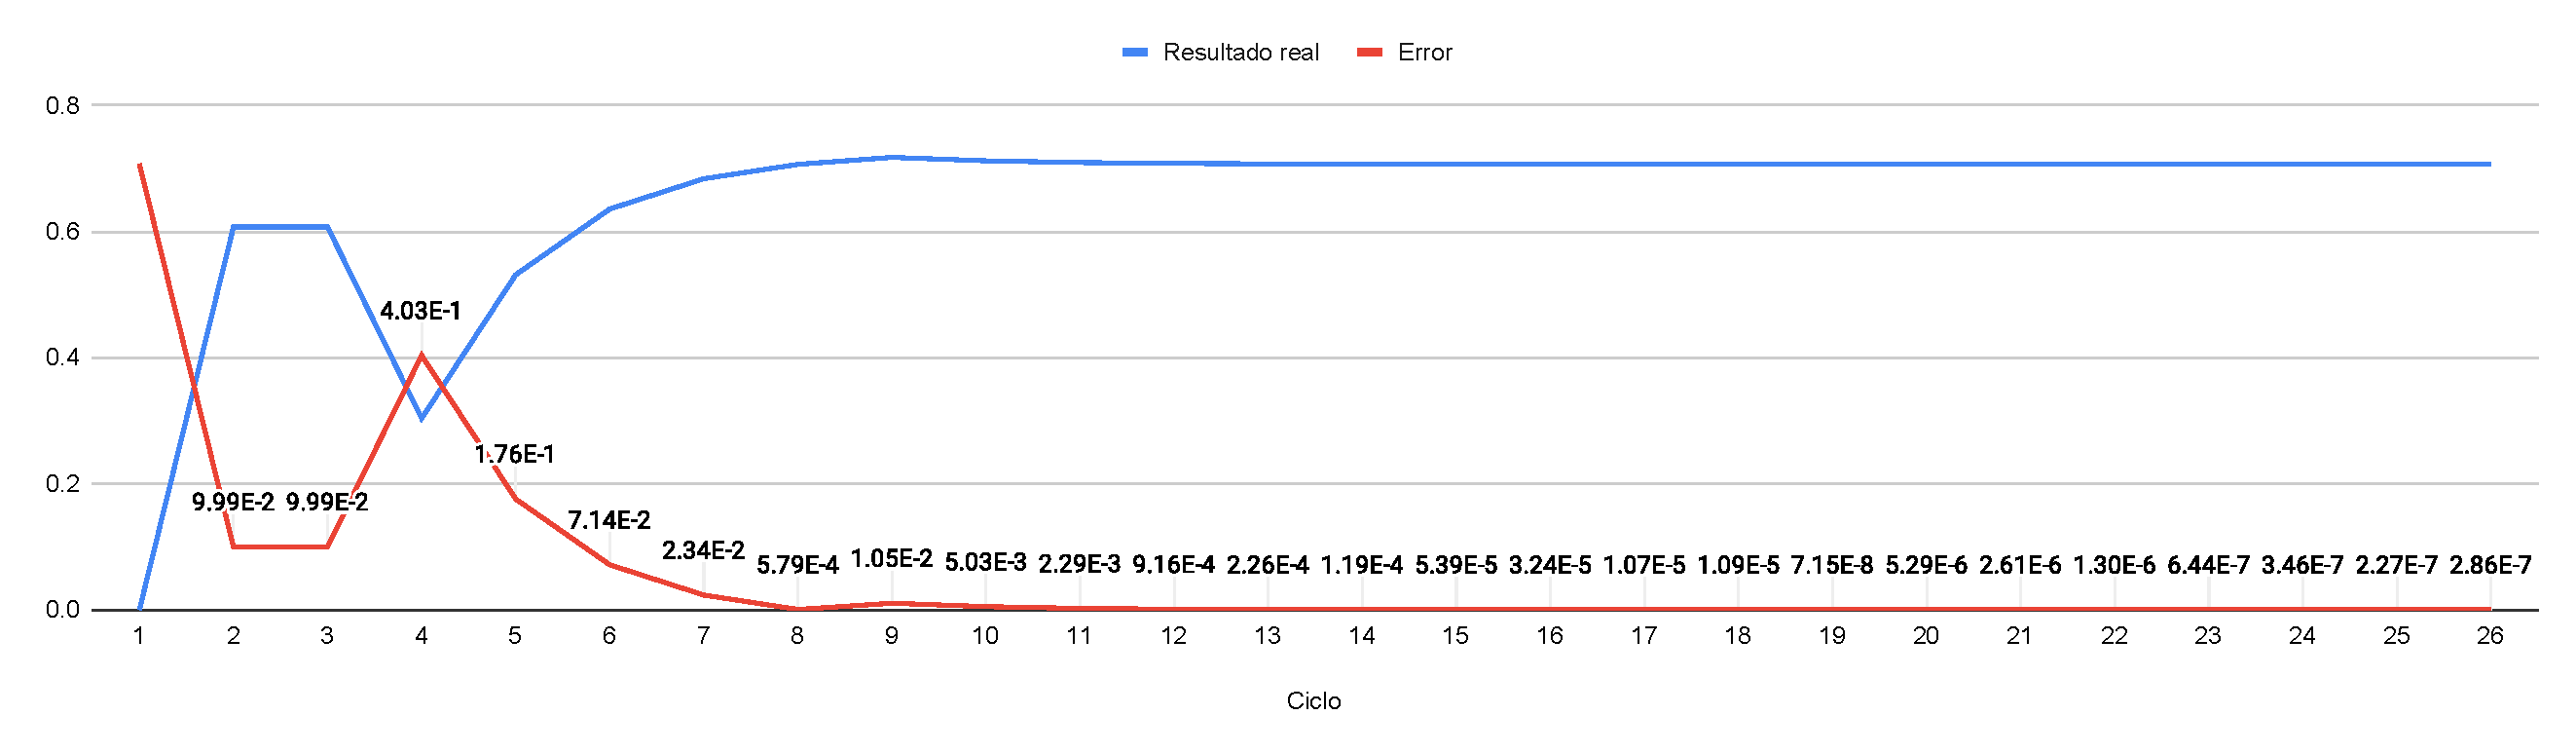
\includegraphics[width=\textwidth]{archivos/CORDIC/real_error2.pdf}
	\caption{Tasa de error en CORDIC con punto flotante.}
	\label{graf:real_error}
\end{figure}


\begin{figure}[H]
	\centering
	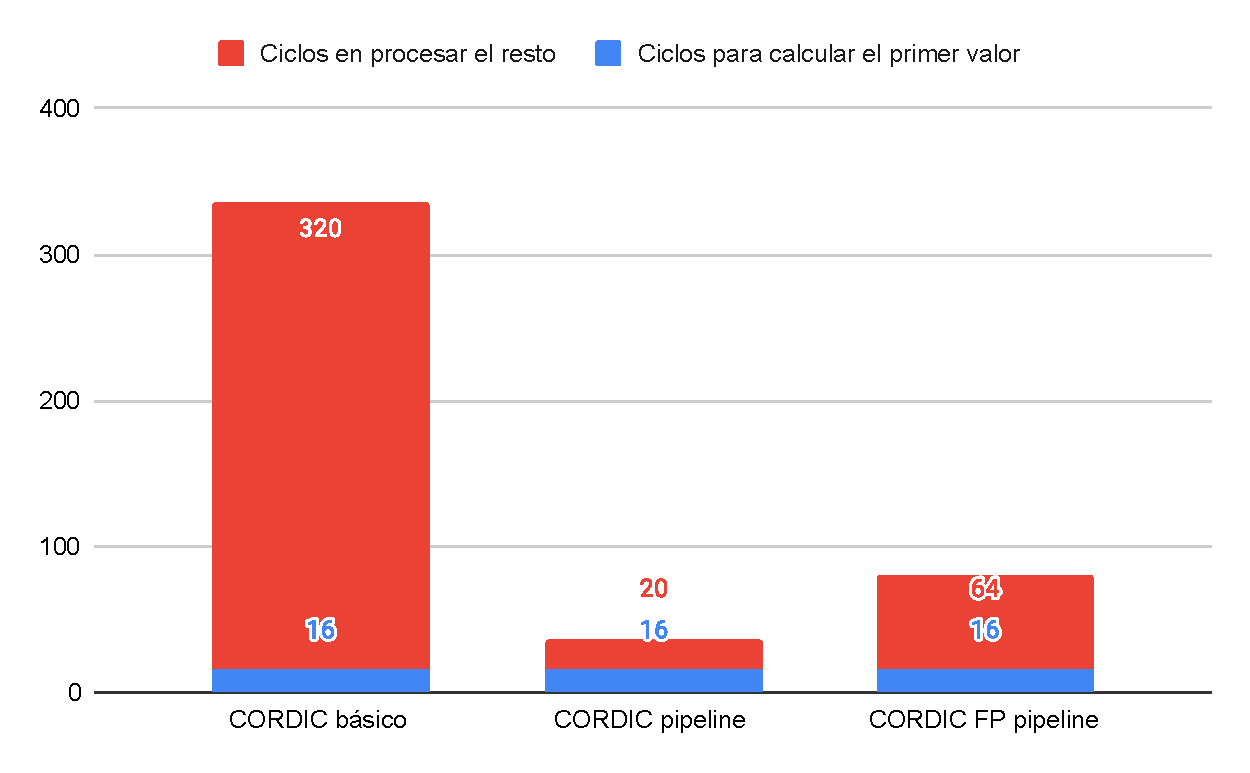
\includegraphics[width=\textwidth]{archivos/CORDIC/ciclos.pdf}
	\caption{Número de ciclos para calcular 20 valores de forma consecutiva (cada ciclo se introduce un nuevo valor).}
	\label{graf:ciclos}
\end{figure}

En la figura \ref{graf:ciclos} se muestra las tres implementaciones desarrolladas anteriormente. Se hace una comparativa con un ejemplo de cálculo de 20 valores consecutivos. Cada ciclo se introduce un nuevo valor en las implementaciones con \textit{pipelining} y en la básica se espera hasta recibir el valor final. Como se puede ver, el número de ciclos para cálcular múltiples valores de forma consecutiva baja drásticamente. Aún con el \textit{overhead} que conlleva calcular el valor en punto flotante, tenemos una reducción muy significativa del tiempo respecto al método básico.
